\section{Discrete distributions}\label{sec:discrete-distrib}
This section briefly reviews the characteristics of some of the
important discrete distributions encountered in practice.
For each distribution, we describe properties and generating
mechanisms, and show how its parameters can be estimated
and how to plot the frequency distribution.
For more detailed information on these and other discrete distributions,
\citet{Johnson-etal:92} present the most comprehensive treatment
and \citet[\C 2]{Zelterman:99} gives a compact summary.

\subsection{The binomial distribution}
\ix{binomial distribution|(}
The binomial distribution arises as the distribution of the
number of events of interest which occur in $n$ independent trials
when the probability of the event on any one trial is the constant
value $p = \Pr ( \textrm{event} )$.
For example, if 15\% of the population has red hair,
the number of red-heads in randomly sampled groups of $n=10$
might follow a binomial distribution, $\Bin(10, 0.15)$.
Over $n$ independent trials, the number of events  $k$
may range from 0 to $n$; if $X$ is a random variable
with a binomial distribution, the probability that $X = k$ is given
by

\begin{equation}\label{eq:binom}
\Bin(n,p): \Pr \{ X = k \} \equiv p ( k )  =
{n \choose k} p^k (1-p)^{n-k}
  \quad\quad k = 0, 1, \dots, n
  \comma
\end{equation}
where ${n \choose k} = n! / k! (n - k)!$ is the number of ways
of choosing $k$ out of $n$.
The first three (central) moments of the binomial distribution are
(letting $q = 1 - p$),
\begin{eqnarray*}
\textrm{Mean}[X] & = & n p  \\
\textrm{Var}[X] &  = & n p q \\
\textrm{Skew}[X] & = & n p q (q - p) 
\comma
\end{eqnarray*}
so the binomial distribution has its maximum variance and is
symmetric when $p = .5$.

If we are given data in the form of a discrete (binomial) distribution
(and $n$ is known),
then the maximum likelihood estimator of $p$ can be obtained
as
\begin{equation*}% \label{eq:binp}
\hat{p} = \frac{\bar{x}}{n} =
  \frac{(\sum_{k} k \times n_k ) / \sum_k n_k}{n}
  \comma
\end{equation*}
with sampling variance $pq/n$.

\subsubsection{Calculation and visualization}
\ix{binomial distribution!visualization|(}
In SAS you can calculate binomial probabilities \eqref{eq:binom} with the
\FUNC{probbnml} and generate random data from a binomial
distribution with the \FUNC{ranbin} or the \CALL{ranbin}.
The \FUNC{probbnml},
\texttt{probbnml(p,n,m)} calculates cumulative probabilities,
$ \sum_{k=0}^{k=m} p ( k )$,
so to find individual probability densities, you must subtract
successive values for $k$ and $k-1$.
In \sasver{6.12} and above, the general \FUNC{pdf}
calculates probability densities directly, for the binomial
and most other distributions.  For the binomial distribution,
it is called as \texttt{pdf('binomial',m,p,n)}.

Discrete distributions are easily visualized by plotting the probability
density (or expected frequencies in a total sample of given size)
against the random variable ($k$), for given values of the distribution
parameters.

For example, assume that 15\% of the population has red
hair, and 35\% has brown hair.
What are the probabilities that in groups of $n=10$
people, $k = 0, 1, \dots, 10$ will have red hair or brown
hair, respectively?
We can calculate these probabilities
(and the expected frequencies in 1000 repetitions) in a \Dstp{} as
follows, giving the output in \outref{out:binomial1}.
We use macro variables for $n$ and $p$ (in the form of a \texttt{DO} list)
so that the same program may be
used for any binomial distributions.
A complete distribution is generated for each combination of $n$ and $p$.

%% input: /users/faculty/friendly/sasuser/catdata/binomial.sas
%% last modified: 22-Dec-97  9:44
\begin{listing}
%let N=10;
%let p=.15, .35;
title "Binomial distributions, N=&N, p=&p";
data binomial;
   reps = 1000;
   drop reps;
   N=&N;
   do p=&p;
      do k=0 to N;
         if k=0 
            then prob = probbnml(p, N, 0);
            else prob = probbnml(p, N, k) - probbnml(p, N, k-1);
         freq = reps * prob;
         output;
         end;
      end;
   label freq='Frequency'
      k = 'k';
proc print;
   id p;
   by p;
run;

proc means data=binomial mean var max vardef=weight;
   var k;
   weight prob;
   by p;
\end{listing}


\begin{Output}
\caption{Binomial probabilities}\label{out:binomial1}
\verbatiminput{ch2/out/binomial1.out}
\end{Output}

\begin{Output}
\caption{Means and variances for binomial probabilities}\label{out:binomial2}
\verbatiminput{ch2/out/binomial2.out}
\end{Output}

Notice that in the \PROC{MEANS} step the option \texttt{VARDEF=WEIGHT}
is used to calculate the variance correctly from a grouped frequency distribution,
producing the output in \outref{out:binomial2}.
These distributions are shown side-by-side in \figref{fig:binomial},
plotted using \PROC{GCHART}, with $p$ as a group variable:
\begin{listing}
proc gchart data=binomial;
   vbar k /sumvar=freq group=p midpoints=0 to 10
      coutline=black frame raxis=axis1;
   pattern1 v=solid c=grayc0;
   axis1 order=(0 to 350 by 50);
run; quit;
\end{listing}

%% one figure
\begin{figure}[htb]
%  \SASfig{binomial.eps}{scale=.75}{binomial}{Binomial distributions for $n=10$ trials}
  \centering
  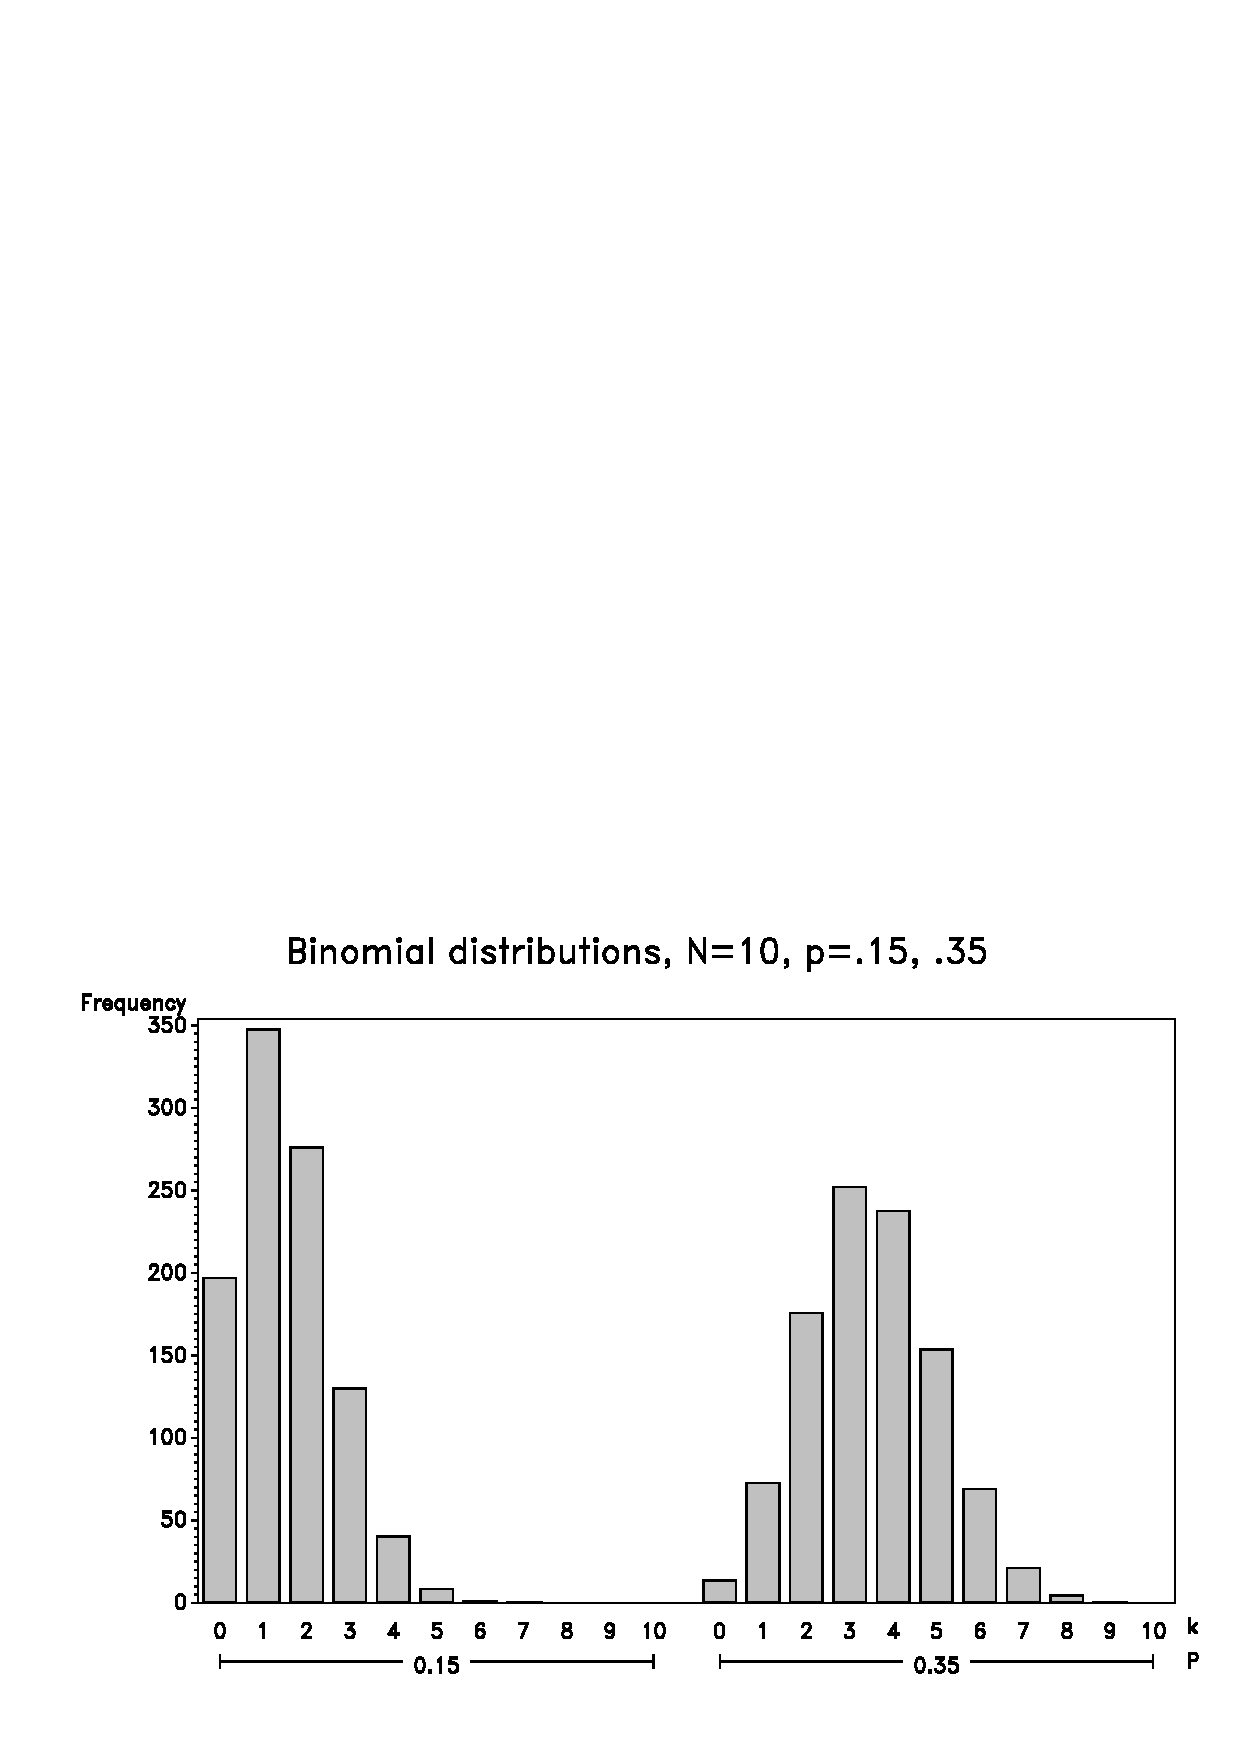
\includegraphics[scale=.75]{binomial}\graphicsfile{ch2/fig/binomial.eps}{}
  \caption{Binomial distributions for $n=10$ trials}%
  \label{fig:binomial}
\end{figure}
Alternatively, one may prefer to plot such distributions as frequency
polygons or as needle graphs, using \PROC{GPLOT}.
For example, \figref{fig:binomial2} shows frequency polygons for
the binomial distributions $\Bin(10,p)$ with $p = 0.15 (0.20) 0.75$,
obtained by running the \texttt{binomial} \Dstp\ with
\begin{listing}
%let p=.15 to .75 by .20;
\end{listing}
The \PROC{GPLOT} step (excluding statements for symbols, axes, and the
legend) is just
\begin{listing}
proc gplot data=binomial;
   plot freq * k = p / frame vminor=1 hminor=0 ... ;
\end{listing}

%% one figure
\begin{figure}[htb]
%  \SASfig{binomial2.eps}{scale=.75}{binomial2}{Binomial distributions for $n=10$ trials, as frequency polygons}
  \centering
  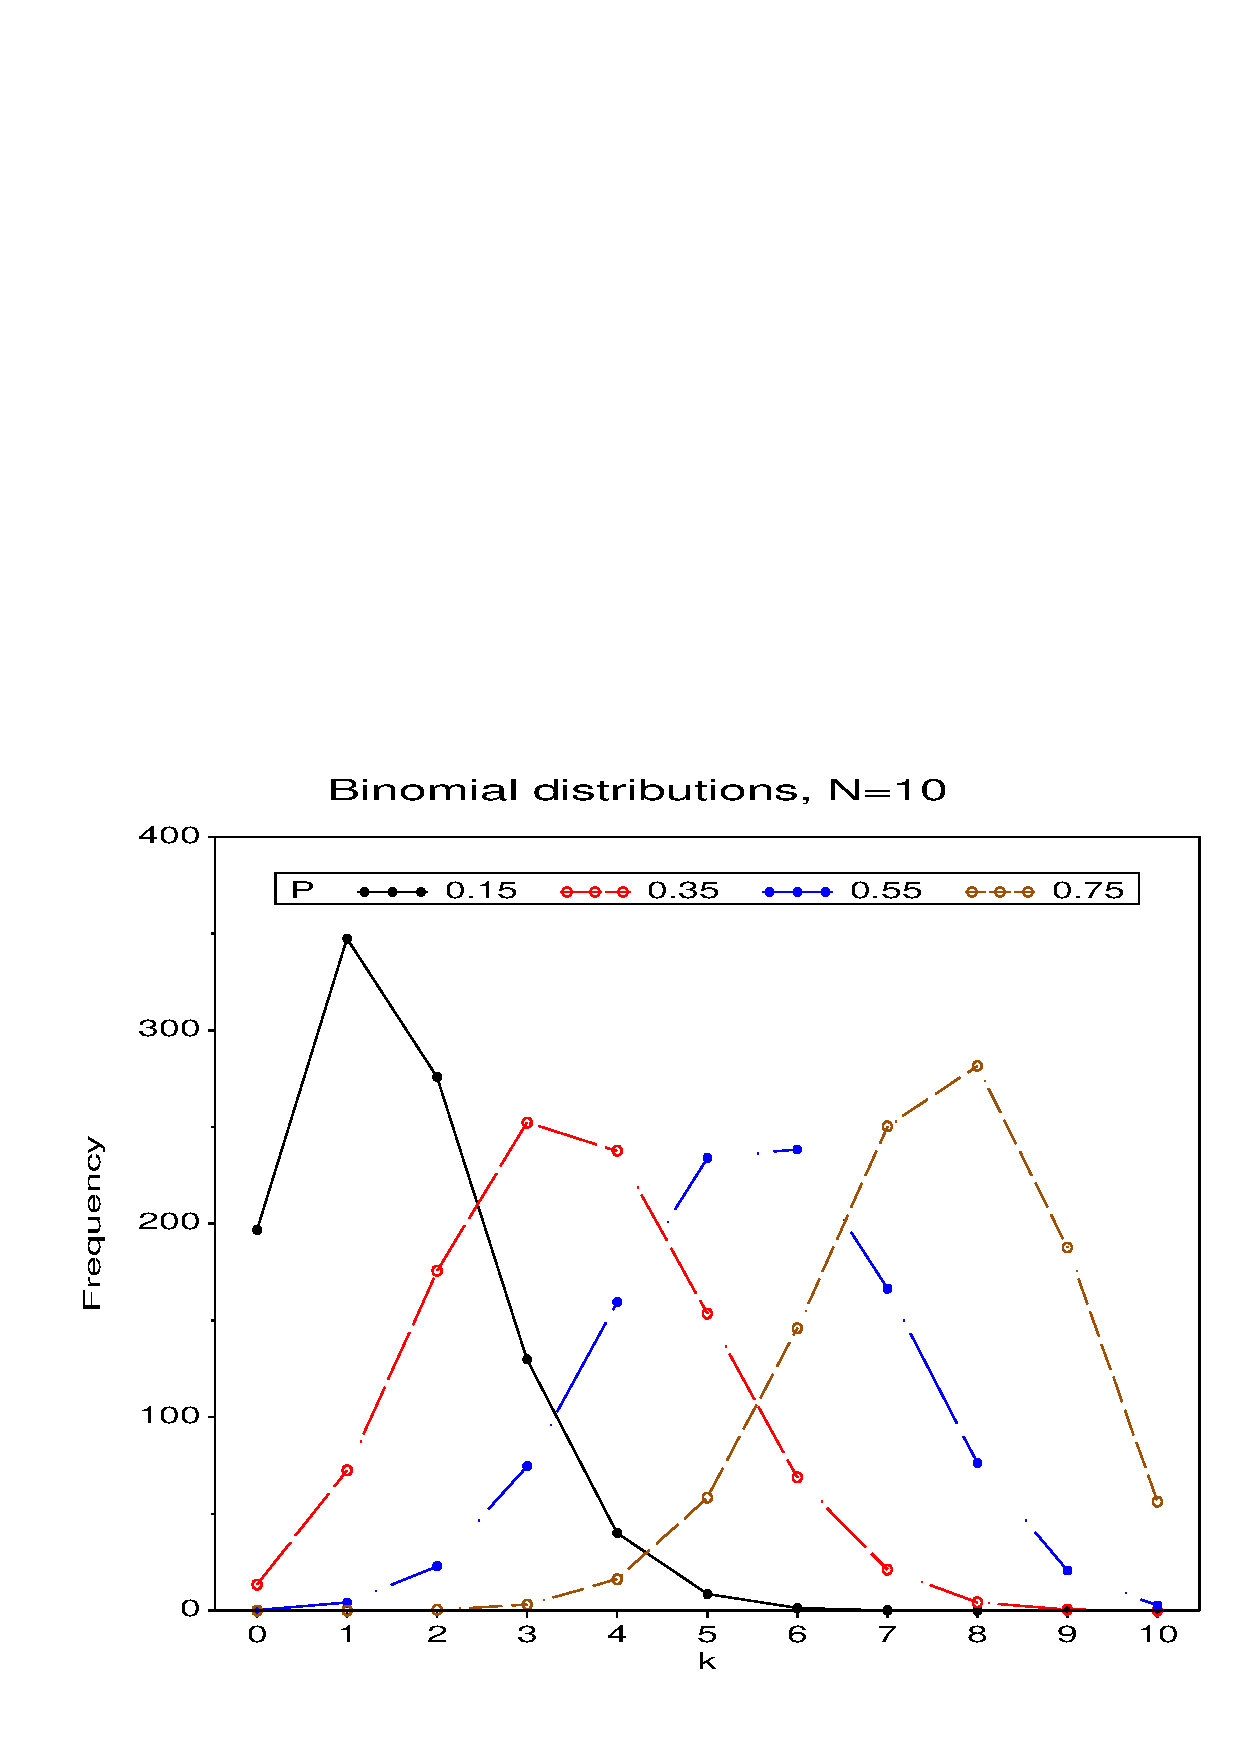
\includegraphics[scale=.75]{binomial2}\graphicsfile{ch2/fig/binomial2.eps}{}
  \caption{Binomial distributions for $n=10$ trials, as frequency polygons}%
  \label{fig:binomial2}
\end{figure}
\ix{binomial distribution!visualization|)}
\ix{binomial distribution|)}

\subsection{The Poisson distribution}
\ix{Poisson distribution|(}

The Poisson distribution gives the probability of an event occurring
$k = 0, 1, 2, \dots$ times over a large number of ``trials'',
when the probability, $p$, that the event occurs on any one
trial is very small and constant;
hence, the Poisson distribution is usually applied to the study of
rare events such as highway accidents at a particular location,
deaths from horse kicks, or defects in a well-controlled manufacturing
process.

For the \IX{Poisson distribution}, the probability function
is
\begin{equation}\label{eq:poisf}
\textrm{Pois}(\lambda):\Pr \{ X = k \} \equiv p (k)=
  \frac{ e^{ - \lambda } \:  \lambda^k } { k ! }
  \quad\quad k = 0, 1, \dots
\end{equation}
where the parameter, $\lambda$ turns out to be the mean of the
distribution.
The first three (central) moments of the Poisson distribution are
in fact all equal to $\lambda$:
\begin{eqnarray*}
\textrm{Mean}[X] & = & \lambda \\
\textrm{Var}[X] &  = & \lambda \\
\textrm{Skew}[X] & = & \lambda 
\end{eqnarray*}
%% Mathematica gives Skew = 1 / \sqrt(\lambda) ???

So, the mean and variance of the Poisson distribution are always
the same, which is sometimes used to identify a distribution
as Poisson.  For the binomial distribution, the mean ($Np$) is always
greater than the variance ($Npq$); for other distributions
(negative binomial and geometric) the mean is less than the
variance.

The maximum likelihood estimator of the parameter \(\lambda\)
in \eqref{eq:poisf} is just
the mean of the distribution,
\begin{equation*}
  \hat{\lambda}= \bar{x} = \frac{\sum_k k \,  n_k}{\sum_k  n_k}
  \period
\end{equation*}
Hence, the expected frequencies can be estimated by substituting the
sample mean into \eqref{eq:poisf}.
Moreover, Poisson variables have a nice reproductive property:
 if $X_1, X_2, \dots X_m$ are independent Poisson
variables with the same parameter $\lambda$, then their
sum, $\sum X_i$ is a Poisson variate with parameter $m \lambda$;
if the Poisson parameters differ, the sum is still Poisson with
parameter $\sum \lambda_i$.

\begin{Example}[soccer]{UK Soccer scores}
\tabref{tab:soccer1}  gives the distributions of goals scored by
the 20 teams in the  1995/96 season of the
 Premier League of the UK Football Association
as presented by
\citet{Lee:97}.%
\footnote{\citet[p. 16]{Lee:97} apparently has the home and away labels reversed in
his table.
The row and column labels in \tabref{tab:soccer1} give means of 1.48
for home teams and 1.06 for away teams.  The raw data were verified
from that listed at \url{http://users.aol.com/mabstabs/soccer.html}}
Over a season
each team plays each other team exactly once, so there are a total of
$20 \times 19 = 380$ games.
Because there may be an advantage for the home team,
the goals scored have been classified as ``home team'' goals
and ``away team'' goals in the table.
%% input: /users/faculty/friendly/sasuser/catdata/soccer1.sas
%% last modified: 09-Jan-98 16:32
\begin{listing}
title 'UK Soccer scores 95/96 season';
data soccer;
   input away @;
   do home = 0 to 4;
      total = home+away;
      input freq @;
      output;
      end;
datalines;
0   27 29 10  8  2
1   59 53 14 12  4
2   28 32 14 12  4
3   19 14  7  4  1
4    7  8 10  2  0
;
proc freq;
   weight freq;
   tables total;
run;

proc means mean var vardef=weight;
   var away home total;
   weight freq;
\end{listing}


If we assume that in any small interval of time there is a small, constant
probability that the home team or the away team may score a goal,
the distributions of the goals scored by home teams
(the row totals in \tabref{tab:soccer1})
may be modeled as Pois($\lambda_H$) and the distribution of
the goals scored by away teams (the column totals)
may be modeled as Pois($\lambda_A$).

If the number of goals scored by the home and away teams are independent%
\footnote{This question
is examined visually in \chref{ch:mosaic} (\exref{ex:soccer2})
and \chref{ch:corresp} (\exref{ex:soccer3}), where we find that the answer
is ``basically, yes''.},
we would expect that the total number of goals scored in any
game would be distributed as Pois($\lambda_H + \lambda_A$).
These totals are shown in \tabref{tab:soccer2}.
As preliminary check of the distributions for the home and away goals,
we can determine if the means and variances are reasonably close
to each other.
If so, then the total goals variable should also have a mean and variance
equal to the sum of those statistics for the home and away goals.
\begin{table}[!hb]
\caption{Total goals scored in 380 games in the Premier
Football League, 1995/95 season}
\label{tab:soccer2}
\vspace{.1in}
\begin{center}
\begin{tabular}{l|rrrr rrrr}
\hline
Total goals      &  0  &  1  &  2  &  3  &  4  &  5  &  6  &  7  \\
\hline
Number of games  & 27  & 88  & 91  & 73  & 49  & 31  & 18  &  3  \\
  \hline
\end{tabular}
\end{center}
\end{table}


The statements below read the data from \tabref{tab:soccer1}, calculate
the \texttt{TOTAL} goals, and find the distribution of \texttt{TOTAL} goals
shown in \tabref{tab:soccer2}.  The \PROC{MEANS} step produces the
mean and variance of each variable, shown in \outref{out:soccer1.2}.
%% input: /users/faculty/friendly/sasuser/catdata/soccer1.sas
%% last modified: 09-Jan-98 16:32
\begin{listing}
title 'UK Soccer scores 95/96 season';
data soccer;
   input away @;
   do home = 0 to 4;
      total = home+away;
      input freq @;
      output;
      end;
datalines;
0   27 29 10  8  2
1   59 53 14 12  4
2   28 32 14 12  4
3   19 14  7  4  1
4    7  8 10  2  0
;
proc freq;
   weight freq;
   tables total;
run;

proc means mean var vardef=weight;
   var away home total;
   weight freq;
\end{listing}


\begin{Output}[htb]
\caption{UK Soccer data, assessing Poissonness}\label{out:soccer1.2}
\small
\verbatiminput{ch2/out/soccer1.2}
\end{Output}
The means are all approximately equal to the corresponding variances.
More to the point, the variance of the \texttt{TOTAL} score
is approximately equal to the sum of the individual variances.
Note also there does appear to be an advantage for the home team,
of nearly half a goal.
\end{Example}


\subsubsection{Calculation and visualization}
\ix{Poisson distribution!visualization|(}
Poisson probabilities may be calculated using the \FUNC{poisson},
which is called as \texttt{poisson(lambda, m)} for a distribution
with mean \texttt{lambda}.
This also returns cumulative probabilities,
$ \sum_{k=0}^{k=m} p ( k )$,
which must be differenced to calculate the probability of exactly
$m$ events.  The \FUNC{pdf}, called as \texttt{pdf('poisson', m, lambda)}
calculates these densities directly.
Random data from a poisson distribution may be obtained using the
\CALL{ranpoi}.

The \Dstp\ below illustrates the use of the \FUNC{pdf} to calculate
poisson frequencies for the distributions with means ($\lambda$) 2 and 5,
for $k = 0, 1, \dots , 12$.

%% input: /Users/friendly/sasuser/catdata/poisson1.sas
%% last modified: 07-Jul-99 13:37
\begin{listing}
%let N=12;
%let lambda = 2, 5;
title "Poisson distributions, lambda=&lambda, k=0..&N";
data poisson;
   reps = 1000;
   drop reps;
   N=&N;
   do lambda=&lambda;
      do k=0 to N;
         prob = pdf('poisson', k, lambda);
         freq = reps * prob;
         output;
         end;
      end;
   label freq='Frequency'
        lambda='Lambda'
        k = 'k';
\end{listing}

\begin{figure}[htb]
  \centering
  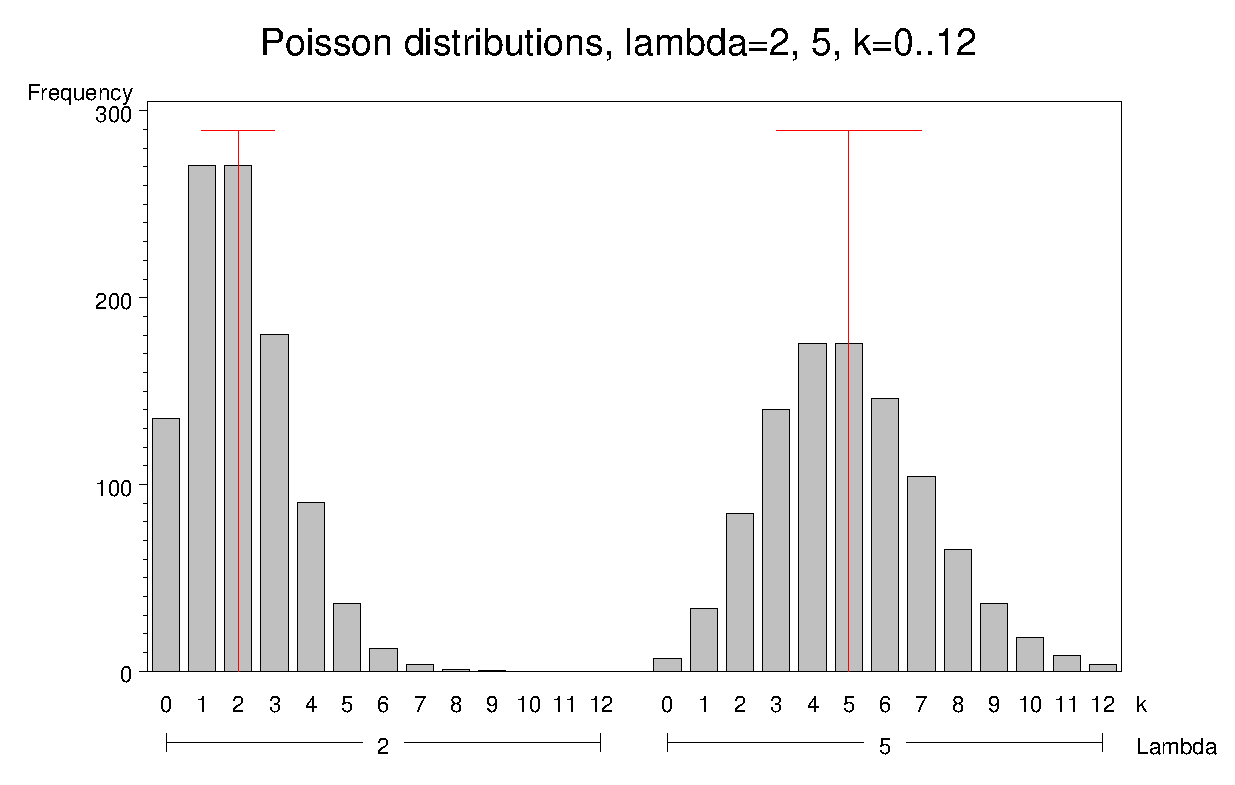
\includegraphics[scale=.75]{poisson1}\graphicsfile{ch2/fig/poisson1.eps}{}
  \caption[Poisson distributions with $\lambda =$ 2, 5.]{Poisson distributions with $\lambda =$ 2 and 5.  The vertical line shows the mean
  of each distribution; the horizontal lines show the standard deviation.}%
  \label{fig:poisson1}
\end{figure}

These distributions are shown in \figref{fig:poisson1},
plotted using \PROC{GCHART} as shown earlier for the binomial
distribution.
\ix{Poisson distribution!visualization|)}
\ix{Poisson distribution|)}

\subsection{The negative binomial distribution}
\ix{negative binomial distribution|(}

The negative binomial distribution is a type of waiting-time distribution.
One form of
the negative binomial distribution
(also called the Pascal distribution) arises when a series of Bernoulli
trials is observed with constant probability $p$ of some event,
and we ask how many trials it takes to observe
$n$ events.
The probability function with parameters $n$ (an integer, $0 < n < \infty$) and $p \, (0 < p < 1)$
gives the probability that $k$ non-events (failures) are observed before
the $n$-th event (success), and
can be written
\begin{equation}\label{eq:negbinf}
\NBin(n,p):   \Pr \{ X = k \} \equiv p(k)  =
  {n+k-1 \choose k} p^n (1-p)^k
  \quad\quad k = 0, 1, \dots , \infty
\end{equation}

The moments of the negative binomial distribution are:
\begin{eqnarray*}
\textrm{Mean}[X] &=&nq / p \\
\textrm{Var}[X] &=&nq / p^2 \\
\textrm{Skew}[X] &=&\frac{2-p}{\sqrt{nq}}
\comma
\end{eqnarray*}
where $q=1-p$.

A more general form of the negative binomial distribution
allows $n$ to take non-integer values and to be an unknown
parameter.
In this case, the combinatorial coefficient,
${n+k-1 \choose k}$ in \eqref{eq:negbinf} is calculated using
the gamma function, $\Gamma(\bullet)$,
a generalization of the factorial for non-integer values,
defined so that $\Gamma(x+1) = x!$ when $x$ is an integer.
Then the probability function \eqref{eq:negbinf} becomes
\begin{equation}\label{eq:negbinf2}
  \Pr \{ X = k \} \equiv p(k)  =
  \frac{\Gamma(n+k)}{\Gamma(n) \Gamma(k+1)}
   p^n (1-p)^k
  \quad\quad k = 0, 1, \dots , \infty
  \period
\end{equation}

In this form, the negative binomial distribution is frequently used
as an alternative to the Poisson distribution when the assumptions
of the Poisson (constant probability and independence) are not
satisfied, or when the variance of the distribution is greater
than the mean (termed \glossterm{overdispersion}).
\citet{GreenwoodYule:20}
developed the negative binomial distribution as a model for
accident proneness or susceptibility of individuals to
repeated attacks of disease.
They assumed that for any individual the number of accidents
or disease occurrences has a Poisson distribution with parameter
$\lambda_i$.
If individuals vary in proneness, so that the $\lambda_i$ have
a gamma distribution, the resulting distribution is the
negative binomial.

When both $n$ and $p$ are treated as unknown parameters,
maximum likelihood estimators are available, but involve
complex non-linear equations.
The simpler method of moments estimators
are
\begin{eqnarray*}
  \hat{p} & = & \bar{x} / s^2 \\
  \hat{n} & = & \bar{x}^2 / ( s^2 - \bar{x} )
  \comma
\end{eqnarray*}
where $\bar{x}$ and $s^2$ are the sample mean and variance of the observed
distribution.
Note that if $s^2 < \bar{x}$, the estimate of $n$ will be negative
and that of $p$ will be greater than 1, so the negative binomial
distribution should be considered inappropriate.

\subsubsection{Calculation and visualization}
The SAS \FUNC{probnegb} calculates negative binomial cumulative probabilities for
integer values of the number of successes parameter, $n$.
To calculate probabilities for individual values of $k$, it is necessary
to compute the difference between successive values $k-1$ and $k$,
as with the binomial and Poisson distribution functions,
or use the \FUNC{pdf}, called as \texttt{pdf('negbinomial', k, p, n)}.
For non-integer values of $n$ it is necessary to calculate the probabilities
directly using \eqref{eq:negbinf2}.
Random values from a negative binomial distribution may be obtained by
calculating the probabilities, $p(k), k=0, 1, \dots$ and
using these with the \FUNC{rantbl}.

\figref{fig:probnegb} shows negative binomial distributions for the number of
trials to observe  $n=2$ or $n=4$ successes with $p = .2, .3, .4$, and
with values of $k$ from 0 to 20.
The vertical line in each panel marks the location of the mean; the horizontal
line shows the range of one standard deviation about the mean.

%% one figure
\begin{figure}[htb]
% \SASfig{probnegb.eps}{scale=.8}{probnegb}{Negative binomial distributions for the number of trials to observe  {\protect{$n=2$ or $n=4$} successes}}
  \centering
  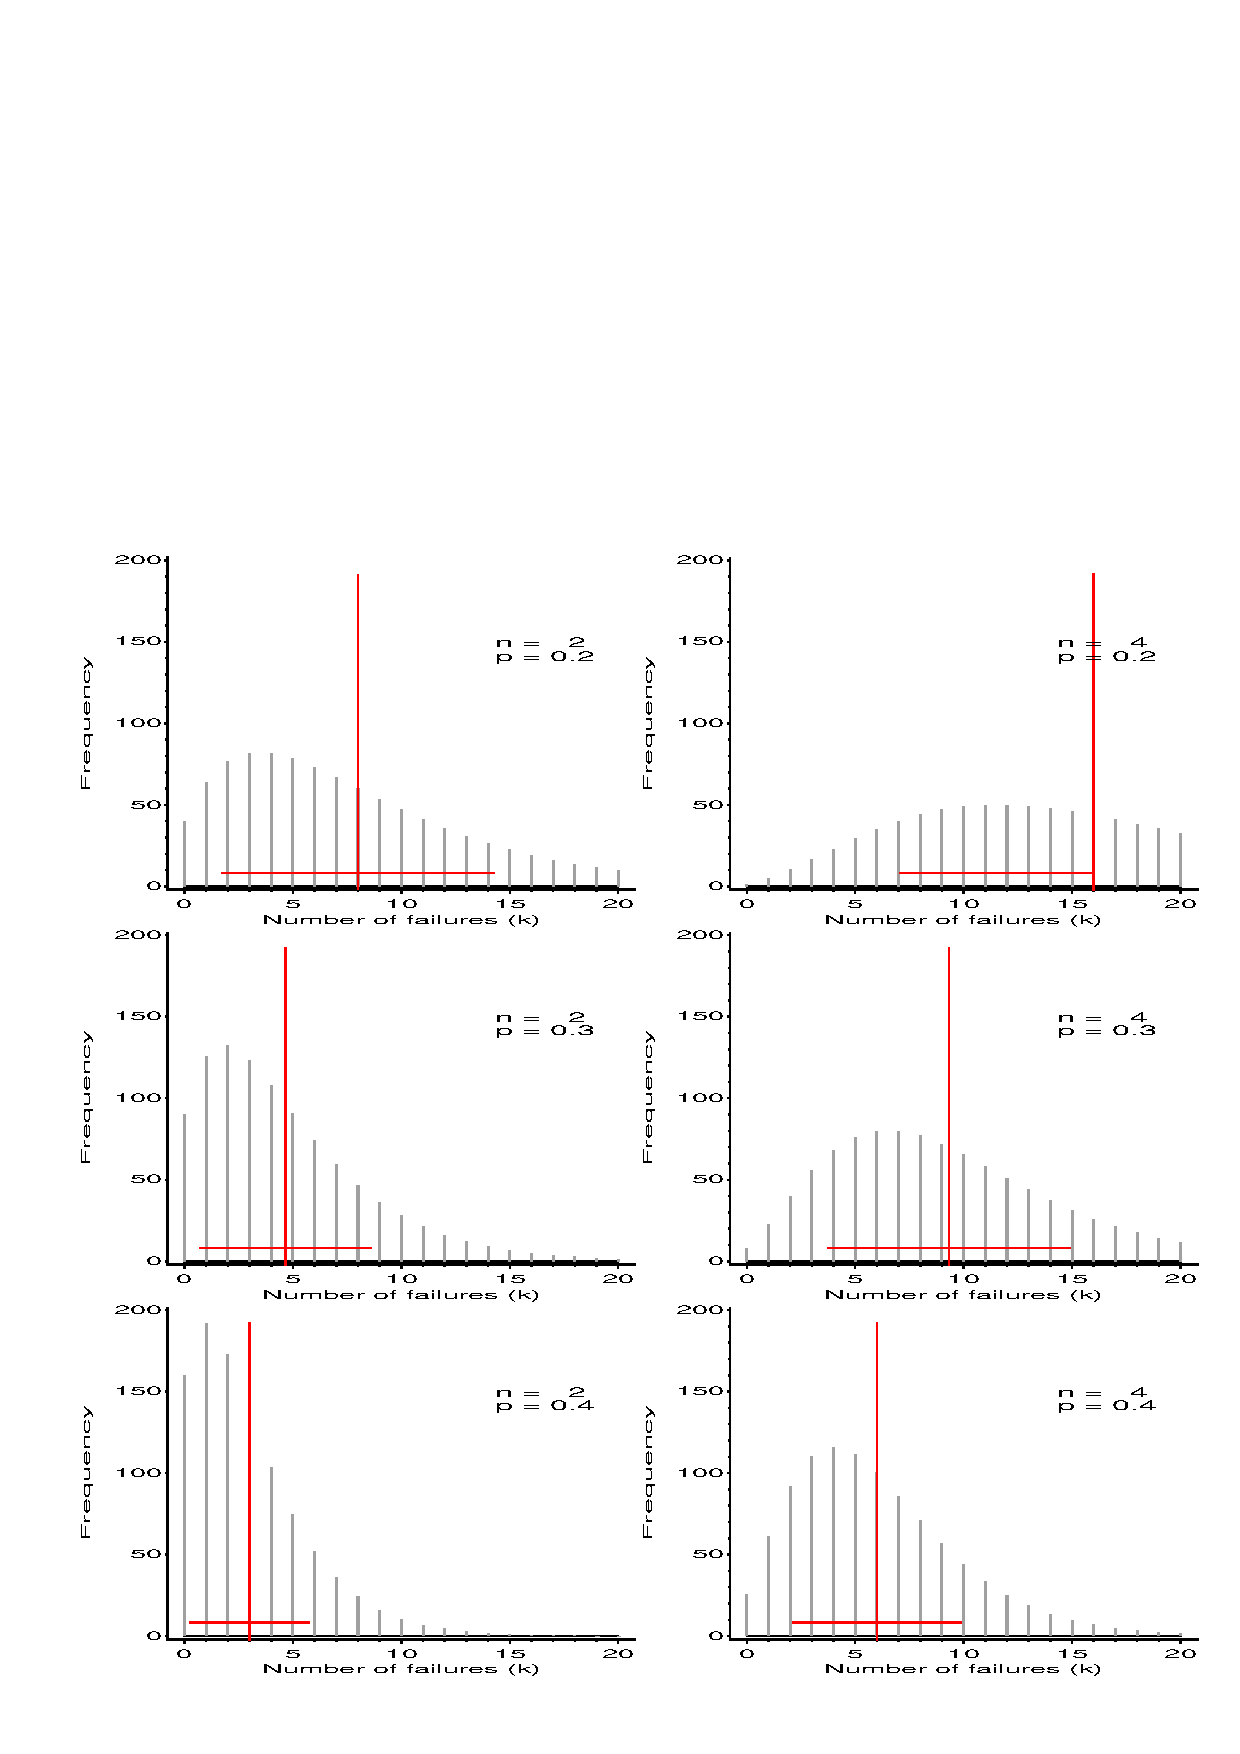
\includegraphics[scale=.8]{probnegb}\graphicsfile{ch2/fig/probnegb.eps}{}
  \caption{Negative binomial distributions for
        the number of trials to observe {\protect{$n=2$ or $n=4$} successes}}%
  \label{fig:probnegb}
\end{figure}
\ix{negative binomial distribution|)}

\subsection{The geometric distribution}
\ix{geometric distribution|(}
The special case of the negative binomial distribution when $n=1$
is a geometric distribution.
We observe a series of independent trials and count the number
of non-events (failures) preceding the first successful event.
The probability that there will be  $k$ failures before the first
success
is given by
\begin{equation}\label{eq:geomf}
\textrm{Geom}(p):   \Pr \{ X = k \} \equiv p ( k )  =
   p (1-p)^k
  \quad\quad k = 0, 1, \dots
  \period
\end{equation}
For this distribution,
\begin{eqnarray*}
\textrm{Mean}[X] & = & 1 / p\\
\textrm{Var}[X] &  = & (1-p) / p^2 \\
\textrm{Skew}[X] & = & (2-p) / \sqrt{1-p}
\end{eqnarray*}
\ix{geometric distribution|)}

\subsection{The logarithmic series distribution}
\ix{logarithmic series distribution|(}
The logarithmic series distribution is a long-tailed distribution
introduced by
\citet{Fisher-etal:43}
in connection with data on the abundance of individuals
classified by species of the type shown for the distribution of butterfly
species
in \tabref{tab:butterfly}.

The probability distribution function with parameter $\theta$ is given by
\begin{equation}\label{eq:logseriesf}
\textrm{LogSer}(\theta): \Pr \{ X = k \} \equiv p ( k )  =
\frac{\theta ^k}{-(k\log (1-\theta ))} =
\alpha \theta^k / k
\quad\quad k = 1, 2, \dots, \infty
\comma
\end{equation}
where $\alpha = -1 / \log(1 - \theta)$
and $0 < \theta <1$.
Fisher derived the logarithmic series distribution by assuming that
for a given species the number of individuals trapped has a Poisson
distribution with parameter $\lambda = \gamma t$, where
$\gamma$ is a parameter of the species (susceptibility to entrapment)
and $t$ is a parameter of the trap.
If different species vary so that the parameter $\gamma$ has a gamma
distribution, then the number of representatives of each species trapped
will have a negative binomial distribution.
However, the observed distribution is necessarily truncated on the left,
because one cannot observe the number of species never caught (where $k=0$).
The logarithmic series distribution thus arises as a limiting form of the
zero-truncated negative binomial.

From \eqref{eq:logseriesf}
\begin{equation*}
\frac{p(k+1)}{p(k)} = \frac{k \theta}{k+1} < 1
\comma
\end{equation*}
for all $k$, since $\theta < 1$.  Hence, the maximum probability occurs at $k=1$
and $p(k)$ decreases steadily as $k$ increases.

The mean and variance of the distribution are
\begin{eqnarray}
\textrm{Mean}[X] & = & \alpha \theta / (1-\theta ) \equiv \mu \label{eq:logsermean}\\
\textrm{Var}[X] & = &  \alpha \theta (1-\alpha\theta) / (1-\theta )^2
= \mu ( \frac{1}{1-\theta} - \mu )
\nonumber
\end{eqnarray}

In fitting this distribution to data, the method of moments and maximum likelihood
both involve equating the sample mean to the population mean in \eqref{eq:logsermean},
a nonlinear equation which must be solved numerically for $\theta$.
When $\bar{x} < 25$, an approximation given by
\citet{Birch:63},
\begin{equation*}%\label{eq:thetabirch}
\hat\theta  \approx
1 - \frac{1}{1 + [ ( \frac{5}{3} - \frac{1}{16}\log \bar{x}) (\bar{x}-1) + 2 ] \log \bar{x} }
\period
\end{equation*}

Another useful unbiased approximation is based on the proportion of observations
at $k=1$,
\begin{equation*}
\hat\theta  \approx 1- \frac{n_1 / N}{\bar{x}}
\period
\end{equation*}
\ix{logarithmic series distribution|)}

\subsection{Power series family}\label{sec:pwrseries}
\ix{power series distributions|(}

I mentioned earlier that the Poisson distribution was unique among all discrete (one parameter) distributions, in that it is the only one whose mean and variance are equal
\citep{Kosambi:49}.
The relation between mean and variance of discrete distributions also provides
the basis for integrating them into a general family.
All of the discrete distributions described in this section are in fact
special cases of a family of discrete distributions
called the power series distributions by
\citet{Noack:50}
and defined by
\begin{equation*}
p(k) = a(k) \theta^k / f(\theta)
\quad\quad k=0, 1, \dots \comma
\end{equation*}
with parameter $\theta > 0$,
where $a(k)$ is a coefficient function depending only on $k$
and $f ( \theta) = \sum_k a(k) \theta^k$ is called the series
function.  The definitions of these functions are shown in
\tabref{tab:pwrseries}.
\begin{table}[!tb] \centering%
\caption{The Power Series family of discrete distributions\label{tab:pwrseries}}%
\small
\begin{tabular}{lllll}\hline
Discrete & Probability  & Series  & Series  & Series \\ 
Distributiion & function, $p(k)$ & parameter, $\theta$ &
function, $f(\theta )$ & coefficient, $a(k)$ \\ \hline
%
Poisson & $e^{-\lambda }\lambda ^k/k!$ & $\theta = \lambda$ & $e^\theta $ & $1/k!$ \\[1ex] 
Binomial & $\binom nkp^k(1-p)^{n-k}$ & $\theta = p / (1-p) $ & $(1+\theta )^n$ & $\binom nk$ \\[1ex] 
Negative binomial & $\binom{n+k-1}kp^n(1-p)^k$ &  $\theta = (1-p) $ & $(1-\theta )^{-k}$ & $%
\binom{n+k-1}k$ \\[1ex] 
Geometric & $p(1-p)^k$ &  $\theta = (1-p)$ & $(1-\theta )^{-k}$ & $1$ \\[1ex]
Logarithmic series & $\theta ^k/[-k\log (1-\theta )]$ &  $\theta = \theta$ & $-\log (1-\theta )$
& $1/k$ \\[1ex] \hline
\end{tabular}
%TCIMACRO{\TeXButton{E}{\end{table}}}
%BeginExpansion
\end{table}%
%EndExpansion



These relations among the discrete distribution provide the basis for
graphical techniques for diagnosing the form of discrete data described
later in this chapter (\secref{sec:discrete-other}).
\ix{power series distributions|)}
